\section{Pebbling Game and Space}
\label{sec:pebbling-game}

%Todo: Discuss relation to resolution space complexity further
Pebbling games denote a family of games played on graphs where nodes are marked and unmarked throughout the rounds of the games.
The goal of these games is to mark some designated node.
On top of the number of rounds played to achieve the goal, an interesting characteristic of a particular instance of a pebbling game is the maximal amount of nodes that are marked simultaneously over the course of all rounds.
The latter characteristic is the one we are interested in, because it models space requirements, when marking a node is interpreted as loading it into memory.
In the context of pebbling games it is common to use the phrase to (un)pebble a node for (un)marking it.

Pebbling games were introduced in the 1970's to model programming language expressiveness \cite{Pippenger1980,Walker1973} and compiler construction \cite{Sethi1975}. 
More recently, pebbling games have been used to investigate various questions in parallel complexity \cite{Chan2013} and proof complexity \cite{Ben-Sasson2009,Esteban2001,Nordstroem2009}. 
They are used to obtain bounds for space- and time-requirements and trade-offs between the two measures \cite{EmdeBoas1979,Ben-Sasson2002}.

There is a variety of different Pebbling Games that differ in the rules and how many types of pebbles are used.
In the following definition we present the Pebbling Game that we use to model space requirements of proofs, which uses a single kind of pebbles.

\begin{definition}[Bounded Pebbling Game]
\label{def:pebbling-game}
The \emph{Bounded Pebbling Game} is played by one player in rounds on a DAG $G = (V,E)$ with one distinguished node $\n \in V$.
The goal of the game is to pebble $\n$, respecting the following rules:
\begin{enumerate}
	\item \label{rule:premises} A node $v \in V$ is pebbleable in a round if and only if all predecessors of $v$ in $G$ are pebbled in this round and $v$ is currently not pebbled.
	\item \label{rule:unpebbling} Pebbled nodes can be unpebbled in any round.
	\item \label{rule:onlyonce} Once a node has been unpebbled, it may not be pebbled in a later round.
\end{enumerate}
%Only pebbled nodes can be unpebbled and only unpebbled nodes can be pebbled.
Every round the player chooses a node $v \in V$, such that $v$ is pebbled or pebbleable.
The \emph{move} of the player in this round is $p(v)$, if $v$ is pebbleable and $u(v)$ if $v$ is pebbled, where $p(.)$ and $u(.)$ correspond to pebbling and unpebbling a node respectively.

\end{definition}

We display examples of this game in Section \ref{sec:algorithms}, when we discuss algorithms to construct strategies for it.

Note that due to rule \ref{rule:premises} the move in each round is uniquely defined by the chosen node $v$.
The distinction of the two kinds of moves is just made for presentation purposes.
Also note that as a consequence of rule \ref{rule:premises}, pebbles can be put on nodes without predecessors at any time.
When playing the Bounded Pebbling Game on a proof $\varphi$, the designated target node is its root.

\begin{definition}[Strategy]
\label{def:strategy}
For a Boundend Pebbling Game, played on a DAG $G = (V,E)$ with distinguished node $\n$, 
a \emph{pebbling strategy} $\sigma$ is a sequence of moves $(\sigma_1,\ldots,\sigma_n)$ of the player such that $\sigma_n = p(\n)$
%A \emph{pebbling strategy} $\sigma$ for the Bounded Pebbling Game, played on a DAG $G = (V,E)$ and distinguished node $\n$, 
%is a sequence of moves $(\sigma_1,\ldots,\sigma_n)$ of the player such that $\sigma_n = p(\n)$.
We denote the set of nodes that are pebbled in round $i$ by 
\begin{align*}
	\pebbledAt{\sigma}{i} \defeq \{ v \in V \mid	& \exists j \leq i: \sigma_j = p(v) \wedge\\
																								&\forall k: j < k \leq i: \sigma_k \neq u(v)\}
\end{align*}
Furthermore, we denote the set of nodes that are ready to be unpebbled in round $i$ by
\begin{align*}
	\unpebbleAt{\sigma}{i} \defeq \{ v \in V \mid	& \nexists j \leq i: \sigma_j = u(v) \wedge\\
																									& \forall c \in \Children{v}{\varphi} c \in \pebbledAt{\sigma}{i}\}
\end{align*}

\end{definition}

The following definition allows to measure how many pebbles are required to play the Bounded Pebbling Game on a given graph.

\begin{definition}[Pebbling number]
The \emph{pebbling number of a pebbling strategy} $(\sigma_1,\ldots,\sigma_n)$ is defined as the maximum number of pebbled nodes in all rounds, 
i.e. $max_{\indexIn{i}{1}{n}}|\pebbledAt{\sigma}{i}|$.
The \emph{pebbling number of a DAG $G$ and distinguished node $\n$} is the minimum pebbling number over all pebbling strategies for $G$ and $\n$.
\end{definition}

The Bounded Pebbling Game from Definition \ref{def:pebbling-game} differs from the Black Pebbling Game discussed in \cite{Hertel2007,Pippenger1982} in two aspects. 
Firstly, the Black Pebbling Game does not include rule \ref{rule:onlyonce}. 
Excluding this rule allows for pebbling strategies with lower pebbling numbers (\cite{Sethi1975} has an example on page 1), at the expense of an exponential upper bound on the number of rounds \cite{EmdeBoas1979}.
Secondly, when pebbling a node in the Black Pebbling Game, one of its predecessors' pebbles can be used instead of a fresh pebble (i.e. a pebble can be moved). 
The trade-off between moving pebbles and using fresh ones is discussed in \cite{EmdeBoas1979}. 
Deciding whether the pebbling number of a graph $G$ and node $\n$ is smaller than $k$ is PSPACE-complete in the absence of rule \ref{rule:onlyonce} \cite{Gilbert1980} and NP-complete when rule \ref{rule:onlyonce} is included \cite{Sethi1975}.

Our interpretation of the game is that every round of the game corresponds to an I/O operation and, if the action of the player is to pebble a node, the processing of the node.
The goal of proof compression is to make proof processing less expensive.
Therefore, admitting exponentially many I/O operations and processing steps in the worst case is not a viable option.
That is the reason why we chose the Bounded Pebbling Game for our purpose.
In the Bounded Pebbling Game the number of rounds is linear in the number of nodes, since every node is pebbled and unpebbled at most once.

In order to process a node according to Definition \ref{def:proof-processing}, the results of processing its premises are used and therefore have to be stored in memory.
The requirement of having premises in memory corresponds to rule \ref{rule:premises} of the Bounded Pebbling Game. 
A node that has been processed can be removed from memory, which corresponds to rule \ref{rule:unpebbling}.
Note that removing a node and its results too early in combination with rule \ref{rule:onlyonce} makes it impossible to process the whole proof.
The optimal moment to remove a node from memory is uniquely determined by the order that nodes are processed (see Theorem \ref{theorem:canonical}).

Definition \ref{def:proof-processing} does not specify in which order to process nodes.
The order in which nodes are processed is essential for the memory consumption, just like the order of pebbling nodes in the pebbling game is essential for the pebbling number.
The following definition allows us to relate pebbling strategies with orderings of nodes.

\begin{definition}[Topological Order]
\label{def:topological-order}
A topological order of a proof $\varphi$ with nodes $V$ is a total order relation $\prec$ on $V$, such that 
$\text{for all } v \in V \text{, for all } p \in \Premises{v}{\varphi}:
p \prec v$.
A sequence of moves $(\sigma_1,\ldots,\sigma_n)$ in the pebbling game \emph{respects} a topological order $\prec$ if for all $j,i \in \{1,\ldots,n\}$ such that $\sigma_j = p(v_j)$ and $\sigma_i = p(v_i)$ it is true that $j < i$ if and only if $v_j \prec v_i$.
\end{definition}

A topological order $\prec$ of a proof $\varphi$ can be represented as a sequence $(v_1,\dots,v_n)$ of proof nodes, by defining $\prec \defeq \{(v_i,v_j) \mid 1 \leq i < j \leq n\}$. 
The requirement that topological orders premises lower than their children corresponds to rule \ref{rule:premises} of the Bounded Pebbling Game.
The antisymmetry together with the fact that $V = \{v_1,\dots,v_n\}$ correspond to rule \ref{rule:onlyonce}.
Theorem \ref{theorem:canonical} shows that the rounds for unpebbling moves are predefined by the pebbling moves, when the goal is to find strategies with small pebbling numbers.
Therefore, there is a bijection between topological orders and canonical pebbling strategies.

\begin{definition}[Canonical Topological Pebbling Strategy]
\label{def:canonstrat}
The \emph{canonical topological pebbling strategy} $\sigma$ for a proof $\varphi$, its root node $s$ and a topological order $\prec$ represented as a sequence $(v_1,\dots,v_n)$ is defined recursively:
$$
\begin{array}{l}
\sigma_1 = p(v_1) \\
\sigma_i = 
	\begin{cases}
		%u(v) & \text{ if for all } c \in \Children{v}{\varphi}: \\
		       %& \quad \text{ there exists }k < i, \sigma_k = p(u) \text{ and }\\
					 %& \quad \text{ for all } l: k < l < i, \sigma_l \neq u(v) \\
		%u(v) & \text{ for all } c \in \Children{v}{\varphi} \text{ exists } k < i, \sigma_k = p(u) \text{ and for all }l: k < l < i, \sigma_l \neq u(v) \\
		u(v) & \text{if } \unpebbleAt{\sigma}{i} \neq \emptyset \text{, where} \\
				 & \quad v = min_{\prec}(\unpebbleAt{\sigma}{i}) \\
		p(v) & \text{otherwise, where } \\
				 & \quad v = min_{\prec}(w \mid \text{ for all } l < i: \sigma_l \neq p(w))
	\end{cases}
	%finished(v,i) := \text{ for all} c \in \Children{v}{\varphi} \text{ exists } k < i, \sigma_k = p(u) \text{ and for all } k < l < i, \sigma_l \neq u(v) 
\end{array}
$$
\end{definition}
Intuitively, the strategy pebbles the nodes in the order in which they are given, and as soon as it is possible to unpebble a node it does so immediately.
The following theorem shows that unpebbling moves can be omitted from strategies for the Bounded Pebbling Game, when the goal is to produce strategies with low pebbling numbers.

\begin{theorem}
\label{theorem:canonical}
The canonical pebbling strategy has the minimum pebbling number among all pebbling strategies that respect the topological order $\prec$.
\end{theorem}
\begin{proof}
Let $\sigma = (\sigma_1,\ldots,\sigma_n)$ be the canonical pebbling strategy for $\prec$ and let $\gamma = (\gamma_1,\ldots,\gamma_n)$ be any pebbling strategy respecting $\prec$.

Let $\#P^{\delta}_i$ and $\#U^{\delta}_i$ be the number of pebbling- and unpebbling- moves respectively, performed by $\delta \in \{\sigma,\gamma\}$ up to round $i$ of the game.
Rule \ref{rule:onlyonce} of the Bounded Pebbling Game disallows to play a pebbling move on the same node more than once.
Furthermore, by our definition of unpebbling moves, such moves are only played on nodes that are pebbled in the respective round.
Therefore, we can characterize the number of pebbled nodes in round $i$ by strategy $\delta$ as $|Peb^{\delta}_i| = \#P^{\delta}_i - \#U^{\delta}_i$.

Pebbling and unpebbling moves are the only possible moves and the player is forced to play a move every turn.
Therefore, we have $\#P^{\delta}_i = i - \#U^{\delta}_i$ and $|Peb^{\delta}_i| = i - 2 \#U^{\delta}_i$.

Strategies $\sigma$ and $\gamma$ respect the same topological order $\prec$.
Therefore, nodes are available for unpebbling in the same sequence for the two strategies.
Strategy $\sigma$ prioritizes unpebbling over pebbling moves, i.e. it does the maximum amount of unpebbling moves possible.
Thus for every $i$ we have $\#U^{\sigma}_i \geq \#U^{\gamma}_i$, which implies $|Peb^{\sigma}_i| \leq |Peb^{\gamma}_i|$.
Since we have the property for every $i$, it also holds for the maximum over all $i$, which is the desired property. 

\noindent\qed

%Since the pebbling number (i.e. the maximum number of simultaneously pebbled nodes) is surely reached after a pebbling move, reordering unpebbling move in this manner does not change the pebbling number of the strategy.
%
%Let $i$ be such that $\gamma_i = u(\n)$ for some node $\n \in V$.
%The rules of the pebbling game imply, that in order to unpebble a node, all its children nodes have to be pebbled.
%The canonical strategy prioritizes such unpebbling moves and since we assumed that consecutive unpebbling moves are made in the same order, we have 
%\begin{equation}
	%\label{eq:proof1}
 %\gamma_i = u(\n) \text{ then }\exists k \leq i: \sigma_k = u(\n)
%\end{equation}
%Since pebbling moves are the only alternative to unpebbling moves, $\sigma$ does the minimal amount of pebbling moves, 
%i.e. 
%\begin{equation}
	%\label{eq:proof2}
	%\begin{split}
	%\forall i \in \{1,\ldots,n\}: &|\{j \mid j \leq i \text{ and }\sigma_j = p(u), u \in V\}| \leq \\
	%&|\{j \mid j \leq i \text{ and }\gamma_j = p(u), u \in V\}|
	%\end{split}
%\end{equation}
%
%We define the set of never pe
%
%We now show that for every $i \in \{1,\ldots,n\}$ we have 
%$\pebbledAt{i}{\sigma} \subseteq \pebbledAt{i}{\gamma}$ by induction on $i$.
%\begin{itemize}
%\item Base Case ($i = 1$): Let $\n$ be the minimal node of $V$ w.r.t. $\prec$.
%The first move of both strategies has to be a pebbling move. Since both strategies respect $\prec$, the pebbling move must pebble the minimal node $\n$. Therefore, $\gamma_1 = \sigma_1 = p(\n)$.
%
%\item Inductive Case ($i > 1$): we distinguish four cases:
%\begin{itemize}
%\item Case 1 ($\gamma_i = p(\n)$ and $\sigma_i = u(\n')$ for some $\n, \n' \in V$): then $\pebbledAt{\gamma}{i} = \pebbledAt{\gamma}{i-1} \cup \{\n\}$ and $\pebbledAt{\sigma}{i} = \pebbledAt{\sigma}{i-1} \setminus \{\n'\}$. By induction hypothesis,  $\pebbledAt{\sigma}{i_1} \subseteq \pebbledAt{\gamma}{i-1}$, and hence $\pebbledAt{\sigma}{i} = \pebbledAt{\sigma}{i-1} \setminus \{\n'\} \subset \pebbledAt{\gamma}{i-1} \cup \{\n\} = \pebbledAt{\gamma}{i}$.
%
%\marginpar{ToDo: improve cases 2, 3 and 4 following the style of case 1.}
%
%\item Case 2 ($\gamma_i = p(\n)$ and $\sigma_i = p(\n')$ for some $\n, \n' \in V$): it follows from \ref{eq:proof1} and \ref{eq:proof2} that $\n' \in \pebbledAt{\gamma}{i}$.
%By induction hypothesis, $\pebbledAt{\sigma}{i} = \pebbledAt{\sigma}{i-1} \cup \{\n'\} \subseteq \pebbledAt{\gamma}{i-1} \cup \{\n'\} = \pebbledAt{\gamma}{i}$.
%
%\item Case 3 ($\gamma_i = u(\n)$ and $\sigma_i = p(\n')$ for some $\n, \n' \in V$): then $\pebbledAt{\gamma}{i} = \pebbledAt{\gamma}{i-1} \setminus \{\n\}$.
%From \ref{eq:proof1} it follows that either $\sigma_i = u(\n)$ or $\n \notin \pebbledAt{\sigma}{i-1}$.
%
%\item Case 4 \ldots
%In case $\sigma_i = u(\n')$ for both cases, we have $\pebbledAt{\sigma}{i} = \pebbledAt{\sigma}{i-1} \setminus \{\n'\} \subseteq \pebbledAt{\gamma}{i}$ by induction.
%In case $\sigma_i = p(\n')$, from \ref{eq:proof1} and \ref{eq:proof2} follows that $\n' \in \pebbledAt{\gamma}{i}$ and again we obtain the desired property by induction.
%\end{itemize}
%
%\end{itemize}

%
%Let $\sigma_i' = p(\n)$ for some node $\n \in V$. Then 
%Suppose that the pebbling number of $\gamma$ is strictly smaller than the one of $\sigma$.
%Let $\sigma = (\sigma_1,\ldots,\sigma_n)$ be the canonical pebbling strategy for $\prec$ and let $\gamma = (\gamma_1,\ldots,\gamma_n)$ be a pebbling strategy respecting $\prec$ such that $\sigma \neq \gamma$.
%All the pebbling strategies respecting $\prec$ differ only in the order of unpebbling moves.
%Definition \ref{def:canonstrat} prioritizes unpebbling over pebbling moves.
%The priorization of unpebbling moves in definition \ref{def:canonstrat} implies that the canonical topological pebbling strategy makes unpebbling moves as soon as possible.
%Consider the moment for unpebbling an arbitrary node $v$ in the canonical pebbling strategy. 
%Unpebbling it later could only possibly increase the pebble number. 
%To reduce the pebble number, $v$ would have to be unpebbled earlier than some preceding pebbling move. 
%But, by definition of canonical pebbling strategy, the immediately preceding pebbling move pebbles the last child of $v$ w.r.t. $\prec$. 
%Therefore, unpebbling $v$ earlier would make it impossible for its last child to be pebbled later without violating the rules of the game.

\end{proof}

As a consequence of Theorem \ref{theorem:canonical}, finding pebbling strategies with low pebbling numbers can be reduced to constructing topological orders.
The memory required to process a proof using some topological order can be measured by the pebbling number of the canonical pebbling strategy corresponding to the order.
We are now ready to define another measure on proofs, which we call space.

\begin{definition}[Space of a Proof]
\label{def:space measure}
The \emph{space} $\pspace{\varphi}{\prec}$ 
of a proof $\varphi$ and a topological order $\prec$ is the pebbling number of the canonical topological pebbling strategy of $\varphi$, its root and $\prec$.
\end{definition}

Note that the space $\pspace{\varphi}{\prec}$ of a proof $\varphi$ and a topological order $\prec$ is an abstract idealized approximation of the memory consumption needed by a proof comsumer processing $\varphi$ according to the canonical strategy corresponding to $\prec$. It is a good approximation, because the size of non-leaf nodes can be assumed to be constant, since non-tautological resolvents (cf. Definition \ref{def:resolvent}) are uniquely determined by their premises and do not need to be explicitly stored in memory. Only the size of leaf nodes varies depending on the size of the input clauses they contain.


\begin{example}

Consider the proof displayed in Figure \ref{fig:spaceproof}.
The indices below the proof nodes indicate a topological order that has pebbling number four.
The implicit unpebbling moves are to unpebble node $1$ after pebbling node $3$, as well as unpebbling nodes $2$ and $4$ after pebbling node $5$.
Before unpebbling nodes $2$ and $4$, nodes $2,3,4,5$ are pebbled which is the maximal amount of pebbles placed on the graph at any time.
It is easy to see, that there is no topological order that has a canonical pebbling strategy with a lower pebbling number.

\begin{figure}[!h]

\centering
\begin{tikzpicture}[node distance=2.5cm]
	
	\proofnode[align=center,font=\small]{root}{$\bot$\\$6$};
	\proofnode[above left of=root,align=center,font=\small]{n3}{$a$\\$3$};
	\proofnode[above right of=root,align=center,font=\small]{n5}{$\neg a$\\$5$};
	\proofnode[above left of=n3,align=center,font=\small]{n1}{$a,\neg b$\\$1$};
	\proofnode[above right of=n3,align=center,font=\small]{n2}{$b$\\$2$};
	\proofnode[above right of=n5,align=center,font=\small]{n4}{$\neg a, \neg b$\\$4$};
	\drawchildren{n5}{n2}{n4};
	\drawchildren{root}{n3}{n5};
	\drawchildren{n3}{n1}{n2};
	
\end{tikzpicture}


\caption{A Simple Proof}
\label{fig:spaceproof}
\end{figure}

\end{example}

The problem of compressing the space of a proof $\varphi$ and a topological order $\prec$ is the problem of finding another topological order $\prec'$ such that $\pspace{\varphi}{\prec'} < \pspace{\varphi}{\prec}$. The following theorem shows that the number of possible topological orders is very large and hence, enumeration is not a feasible option when trying to find a good topological order.

\begin{theorem}
\label{theorem:enumeration}
There is a sequence of proofs $(\varphi_1,\varphi_2,\ldots)$ such that $\plength{\varphi_m} \in O(m)$ and $|T(\varphi_m)| \in \Omega(m!)$, where $T(\varphi_m)$ is the set of possible topological orders for $\varphi_m$.
\end{theorem}
\begin{proof}
Let $\varphi_m$ be a perfect binary tree with $m$ axioms. Clearly, $\plength{\varphi_m} = 2m-1$.
Let $(v_1,\ldots,v_n)$ be a topological order for $\varphi_m$. 
Let $\Axioms{\varphi_m} = \{v_{k_1},\ldots,v_{k_m}\}$, then $(v_{k_1},\ldots,v_{k_m},v_{l_1},\ldots,v_{l_{n-m}})$, 
where the indexes are such that $(l_1,\ldots,l_{n-m}) = (1,\ldots,n) \setminus (k_1,\ldots,k_m)$, is a topological order as well. 

Likewise, $(v_{\pi({k_1})},\ldots,v_{\pi({k_m})},v_{l_1},\ldots,v_{l_{n-m}})$ is a topological order, for every permutation $\pi$ of $\{k_1,\ldots,k_m\}$. There are $m!$ such permutations, so the overall number of topological orders is at least factorial in $m$ (and also in $n$).

\noindent\qed
\end{proof}

There might not only be many possible topological orders, their pebbling numbers might also be substantially different.

\begin{theorem}
\label{theorem:enumeration}
There is a sequence of proofs $(\varphi_2,\varphi_4,\ldots)$ such that there are topological orders $\delta, \gamma$ for $\varphi_m$ with pebbling numbers $n_\delta$ and $n_\gamma$, such that $n_\delta = O(2^{n_\gamma})$.
\end{theorem}
\begin{proof}
Again let $\varphi_m$ be a perfect binary tree with $m$ axioms, where $m > 1$.
Let $\delta = (v_{k_1},\ldots,v_{k_m},v_{l_1},\ldots,v_{l_{n-m}})$ be the topological order, where indices are defined as in the proof of Theorem \ref{theorem:enumeration}.
The strategy initially pebbles all axioms, making no node available for unpebbling.
Only after pebbling one additional node, two axioms can be unpebbled.
Therefore, we have that $n_\delta = m + 1$.

Let $\gamma$ be the strategy that processes $\varphi_m$ from left to right.
We show by induction on $m: n_\gamma = \log_2(m)+2$.
The base case is $m = 2$.
The strategy $\gamma$ has to pebble both axioms first, before being able to pebble the root node.
Therefore, we have $n_\gamma = 3 = \log_2(2) + 2$ for $\varphi_2$.

Let $\varphi_m$ be a perfect tree with $m=m'*2$ axioms, which has a left and a right subproof, which are perfect bianry trees with $m'$ axioms.
By induction hypothesis, we have that $\gamma$ needs $\log_2(m') + 2$ pebbles on the left subproof.
One pebble remains on the root of the left subproof, while processing the right subproof.
Therefore, we have $n_\gamma = \log_2(m') + 3 = \log_2(\frac{m}{2}) + 3 = \log_2(m) + 2$ for $\varphi_m$.

We have $n_\delta = m + 1 = O(2^{\log_2(m)+2}) = O(2^{n_\gamma})$.

\noindent\qed
\end{proof}